\cotefile{157-1}
\scanpage{82}
\mspage{\unsure{88|28}}

On pose

\[
X'=S'\times\overline S\qquad X''=S''\times\overline S
\]

\margin{$\overline S$ copie conforme de $S$, cf ci-dessus}

et il faut, pour recoller $X'$ et $X''$, se donner un \unsure{isom|iso} entre $X'\mid\unsure{\Omega|R}\simeq\unsure{\mathbb{T}|T|R|\mathbb{I}}\times\overline S=\unsure{\overline S'|\overline S}\amalg\overline S'$ et $X''\mid\Omega\simeq\mathbb{T}\times\overline S=\unsure{\overline S''|\overline S}\amalg\overline S''$ qui \deleted{\unsure{respecte la}} soit un $T$-foncteur, i.e. qui provienne de deux iso.

\diagram{\begin{tikzcd}[ampersand replacement=\&,row sep=small]
\overline S\arrow[r,"u_a"] \&\overline S\\
\overline S\arrow[r,"u_b",no head]\&\overline S .
\end{tikzcd}}

On prendra \deleted{\unsure{donc|$u_a=$}}

\[
\begin{aligned}
u_a&=\mathrm{id}_{\overline S}\\
u_b&=\text{symétrie p.r. à \unsure{l'axe} $\overline0,\overline{0'}$ i.e.,}\\
&\qquad u_b\text{ laisse fixes }\overline0,\overline{0'}\text{ et intervertit}\\
&\qquad\overline a\text{ et }\overline b .
\end{aligned}
\]

(C'\deleted{\illegible{1}}\inserted{est} plus clair si on \unsure{désidentifie|désidentifiait} la base et la fibre, en prenant fibre $\overline S$ :

\diagram{\begin{tikzcd}[ampersand replacement=\&,row sep=tiny,column sep=small]
\&\overline a\&\\
\overline0\arrow[ur]\arrow[dr]\&\&\overline{0'}\arrow[ul]\arrow[dl]\\
\&\overline b\&
\end{tikzcd}}

)

\deleted{\unsure{Le|Il}} Pour voir que $X$ est une \deleted{\unsure{$\mathscr F$|$f$}} $\mathbb D$-fibration sur $S$ (quel que soit $\mathbb D$) \deleted{en fait il} \inserted{\unsure{prouvons}} \deleted{il suffit de voir} qu'il \unsure{est} \uline{propre} sur $S$ --- \deleted{ce qui \inserted{est}} \unsure{revient|revient à} : voir que $X'\to S'$ et $X''\to S''$ sont propres, ce qui est trivial. \deleted{Il suffit} Pour voir que c'est une \inserted{$\mathbb D$-}fibration, on est également ramené au cas de $X'\to \unsure{S'|O'}$ et $X''\to S''$, où c'est aussi trivial. On a utilisé le

% slanted
\margin{\uline{NB} $f:X\to S$ est également \uline{lisse}, car c'est un \unsure{fibré trivial} (un produit) au-dessus des deux \deleted{\unsure{$+$}} ouverts $S\smallsetminus\{a\}$, $S\smallsetminus\{b\}$, qui recouvrent $S$. Mieux : $f$ est à la fois $\mathit{Cat}$-fibrant et $\mathit{Cat}$-cofibrant (Caractérisation \unsure{infinitésimale} par les propriétés des $X\times_S\Delta^{\unsure{2|n}}\to\Delta^2$, pour $\Delta^2\to S$).}

\uline{Lemme} Soit $f:X\to S$, $(S_i)_{i\in I}$ une famille de sous-\deleted{catégories} fermés recouvrant $S$. $\forall i$, soit $X_i=X_i\times_S S_i\xrightarrow{f_i}S_i$. Pour que $f$ soit propre, il faut et que les $f_i$ le soient. \deleted{Pour que $f$ soit une} $\mathbb D$-fibration propre, il f. et s. que les $f_i$ le soient.

% archive sheet number: 81
\scanpage{83}
\mspage{89}

% slanted
\margin{Mais dans le cas du \unsure{rev.} à 2 feuillets de $S$, il n'y a pas même de calcul à faire !}

Voici \deleted{pourquoi} le \deleted{petit} calcul qui montre que $f:X\to S$ est une $\mathbb D$-équivalence. On fait le calcul en cohomologie, on \unsure{doit|désire} prouver que les

\[
H^{\unsure{\cdot|i}}(S,k)\longrightarrow H^{\cdot}(X,k)
\]

iso (et de $=$ pour tout coeff. constant \deleted{\unsure{sur}} $M$ sur $S$).

Or $H^{\cdot}(X,k)\overset{\mathrm{def}}=R\Gamma_X(k_X)=\unsure{\mathbb R|R}\Gamma_S(Rf_*(k_X))$, et ceci est induit par

\[
i:k_S\unsure{\relbar|\longrightarrow} Rf_*k_X
\]

Or on a

\[
Rf_*k_X\simeq\underbrace{k_S}_{\text{\unsure{im.}}(i)}\oplus
\underbrace{k_S[1]}_{k_S\ \text{en degré }1}^{\text{\uline{tordu}}}\,,
\]

savoir \textquotedblleft tordu\textquotedblright\ par l'action de monodromie de $S=S^1$, laquelle est la symétrie \deleted{\unsure{$-1$}} $\lambda\longmapsto-\lambda$. On a

\[
R\Gamma_S(k_S[1]^{\text{tordu}}\unsure{]|)}=
H^1(\underset{\substack{\parallel\\\mathbb Z}}{\underline{\pi_1(S)}},k^{\text{tordu}}\unsure{)|\}} )=
\underset{\scriptstyle k/(u-\mathrm{id})k}{k_{(\mathbb Z)}}=\underset{\substack{\parallel\\0}}{k/2k}
\]

d'où le résultat.

Notons que si on regarde

\[
X'=X\times_S X\xrightarrow{f'}S\ ,
\]

on aura par Künneth relatif

\[
\begin{aligned}
Rf'_*(k_{X'})&\simeq Rf_*(k_X)\mathbin{\overset{\unsure{\mathbb L|L}}{\otimes}}Rf_*(k_X)\simeq\\
&k_S\oplus k_S[1]^t\oplus k_S[1]^t+
\underbrace{k_S(1)^t\otimes k_S[1)^t}_{\displaystyle k_S[2]^{\text{\uline{n. tordu}}}}\, ,
\end{aligned}
\]

\deleted{\unsure{donc}} d'où

\[
\begin{aligned}
\unsure{R H|H}^{\cdot}_{\mathbb D}(X',k)&\simeq R\Gamma_{X'}(k_{X'})\simeq R\Gamma_S(Rf'_*(k_{X'})\\
&\simeq R\Gamma_S(k_S)\oplus R\Gamma_S(k_S)[2]
\end{aligned}
\]

et $H^{\cdot}_{\mathbb D}(\unsure{S|X},k)\to H^{\cdot}_{\mathbb D}(X',k)$ \unsure{n'est} \uline{pas} iso.

% archive sheet number: 82
\scanpage{84}
\mspage{90}

Ainsi $f:X\longrightarrow S$ qui est une $\mathbb D$-fibration (propre et lisse) satisfait bien les conditions \inserted{\unsure{équiv.}} b), b') de la prop. \unsure{2,|2$_0$} (page 79), mais non la condition a), puisque le changement de base

\diagram{\begin{tikzcd}[ampersand replacement=\&]
X'=X\times_S\unsure{X|V|X'}\arrow[r,"q=\mathrm{pr}_1"]\arrow[d,"f'=\mathrm{pr}_2"'] \&X\arrow[d,"f"]\\
S'=X\arrow[r,"p=f"']\&S
\end{tikzcd}}

est une $\mathbb D$-équivalence $S'\to S$, alors que $X'\to X$ ne l'est pas.

Voici un autre contre'exemple, sur le même principe mais un peu plus simple. Soit $G$ un groupe \deleted{\unsure{fini}} \inserted{fini} (p. ex. $G=\mathbb Z/2\mathbb Z$), faisons le opérer sur une \deleted{catégorie} objet $\unsure{Z|\mathbb Z|X}$ de $\mathit{Cat}$, \unsure{soit|d'où} $S=[G]=B_G$ la catégorie réduite à un objet \inserted{$a$}, avec $G=\mathrm{End}(a)$.

\deleted{Alors on a}

\[
\deleted{f:X\longrightarrow S}
\]

\deleted{je dis que c'est une $\mathbb D$-fibration, propre et lisse, quel que soit $\mathbb D$. \unsure{Pour ceci|Bien plus}, considérons le chgt de base}

\[
\deleted{e\longrightarrow S}
\]

\deleted{\unsure{où}} Soit $E_G$ la catégorie \deleted{\unsure{$(B_G)_{/a}$}} \deleted{\unsure{connue de}} (\unsure{isom} : \deleted{\unsure{$(B_G)_{/a}$}}\inserted{$(B_G)_{/a}$})

\[
\mathrm{Ob}\,E_G=G,\qquad \mathrm{Hom}_{E_G}(g,g')=\{h\in G\mid\deleted{\unsure{h}}g=g'h\},
\]

composition évidente --- donc $E_G$ est un groupoïde trivial (\unsure{0|1}-connexe). Le groupe $G$ \deleted{\unsure{y}} opère à \deleted{droite}\inserted{gauche} librement, \inserted{par translations}, et $B_G=E_{\deleted{\unsure{G}}G}/G$.

% archive sheet number: 83
\scanpage{85}
\mspage{91}

Si $G$ opère à gauche sur $\unsure{Z|\mathbb Z}$, on peut alors l'utiliser pour tordre $Z$, par

\[
X=\unsure{E_G|B_G}\wedge_G Z=(E_G\times Z)/\underset{\text{de }G}{\text{opération ``diagonale''}}
\]

D'où on a un diagramme cartésien

\diagram{\begin{tikzcd}[ampersand replacement=\&,column sep=large,row sep=large]
X^{\unsure{p|\prime|\sharp}}\arrow[d,"f"]\&
\overset{\substack{X'\\ \shortparallel}}{Z\times E_G}\arrow[l]\arrow[d,"\mathrm{pr}_2"]\&
\overset{\substack{X''\\ \shortparallel}}{Z}\arrow[l,dashed,"\overset{\mathbb D}{\sim}"']\arrow[d]\\
\underset{\substack{\shortparallel\\ S}}{B_G}\&\underset{\substack{\shortparallel\\ S'}}{E_G}\arrow[l]\&
\underset{\substack{\shortparallel\\ S''}}{e}\arrow[l,dashed,"\overset{\mathbb D}{\sim}"']
\end{tikzcd}}

\deleted{\unsure{La conclusion}} Comme le chgt de base $\underset{\substack{\shortparallel\\\underbrace{S^{\unsure{\prime|\prime\prime}}=E_G}}}{(B_G)_{/a}}\to\underset{\substack{\shortparallel\\ S}}{B_G}$ transforme $X'\deleted{\unsure{/}}$ sur $B_G$ en produit (lequel est \inserted{un $\mathbb D$-\unsure{fibré|fibr.}} propre et lisse sur $\unsure{E|S}$) on voit que $X'$ sur $B_G$ est \inserted{un $\mathbb D$-\unsure{fibré|fibr.}} propre et lisse\deleted{, et \unsure{comme on}} (car c'est là une condition locale sur $B_G$).

\unsure{\S}

On suppose maintenant que $G$ est fini d'ordre $n>1$, et soit $k$ un anneau où $n$ est inversible, \deleted{Alors \unsure{$H$}} $\mathbb D=\mathrm{Der}\,(k\text{-}\mathrm{Mod})$. Alors $E_G\to B_G$ est une $\mathbb D$-équivalence, \deleted{\unsure{Bien}} ce \deleted{\unsure{contre, $Z$}} qui revient au même $e\to B_G$ \unsure{:} l'est. Pourtant après changmt de base soit par $S'=E_G$, soit par $S''=e$, \deleted{\unsure{la}} $X'\to X$ (ou ce qui revient au même, $X''\unsure{\relbar|\to} X$) n'a \deleted{pas} guère de raison d'en être une. On a en cohomologie

% slanted
\margin{En fait $e,E_G,B_G$ sont $\mathbb D$-asphériques !}

\[
R\Gamma_X(k_X)\simeq R\Gamma_{B_G}(f_*(k_X))\simeq R\Gamma_G(G,H^{\unsure{\cdot|*}}(Z,k))
\]

% archive sheet number: 84
\scanpage{86}
\mspage{92}

donc ($n$ étant inversible dans $k$) :

\[
H^{\unsure{\cdot|i}}(X,k)=R\Gamma_X(k_X)\simeq\deleted{\unsure{R}}H^{\cdot}(Z,k)^G\unsure{\relbar\joinrel\relbar|\longrightarrow}H^*(Z,k)\ ,
\]

ce n'est en général pas un iso. On peut prendre p. ex. $G=\mathbb Z/2\mathbb Z$, $Z\sim S^1$ comme avant, et $G$ opérant par symétrie de $S^1$, comme précédemment.

Cet exemple est particulièrement convainquant, car c'est un exemple \uline{avec} $S,S'$ $\mathbb D$-\uline{asphériques}, et $S'\to S$ un iso. local (en fait, un revêtement principal de $S$).

C'est aussi un exemple d'un $\mathbb D$-fibré lisse \unsure{et|plus} propre $X\to S$, sur une base \uline{asphérique} $S$, et tel que l'inclusion d'une fibre dans $X$

\[
X_s\unsure{\relbar|\longrightarrow}X
\]

ne soit \uline{pas} une $\mathbb D$-équivalence.

Le seul reproche qu'on puisse faire à cet exemple, en comparaison avec le précédent, c'est que les catégories $X,S$ ne sont pas \inserted{des ens.} ordonnés. \inserted{Et} $S$ ne peut être un ensemble ordonné fini, car l'espace classifiant d'un groupe fini a de la cohomologie en toutes dimensions (sauf erreur).

% archive sheet number: 85
\scanpage{87}
\mspage{93}

Mais on peut s'inspirer de cet exemple pour le modifier de façon qu'il se transpose à des ens. ordonnés. Il suffit de réaliser, pour $\unsure{G|C}$ donné

a) Une opération \deleted{\unsure{sans point fixe}}\inserted{\uline{libre} de $G$} sur un \deleted{catégorie}\inserted{objet} $E$ de $\mathit{Cat}$, \deleted{qui soit} \inserted{telle que} \deleted{$\mathbb D$-asphérique (i.e. à la cohomologie triviale)} $H^{\unsure{\cdot|*}}(E,k)^G\simeq k$, i.e. $B=E/G$ soit $\mathbb D$-asphérique

b) Une opération de $G$ sur un objet $Z$, telle que l'inclusion

\[
H^{\cdot}(Z,k)^G\unsure{\relbar\joinrel\relbar|\longrightarrow}H^{\cdot}(Z,k)^G
\]

ne soit pas iso.

c) \deleted{\unsure{D'}}\inserted{Choisir pour $E,Z$ des ens. ordonnés, et} S'assurer que $B=E/G$ est également représenté par une catégorie ordonnée. Sauf erreur, il en sera de $=$ pour $X=E\times Z/G$.

\unsure{Donc|D'où} on aura en tous les cas

\diagram{\begin{tikzcd}[ampersand replacement=\&,row sep=large,column sep=large]
X\arrow[d] \& \overset{\substack{Z\times E\\ \shortparallel}}{X'}\arrow[l]\arrow[d] \& Z\arrow[l]\arrow[d,no head]\\
\underset{\substack{=E/G\\ \text{asph.}}}{S}\&\underset{\substack{=E\\ \text{asph.}\\ \text{si on peut}}}{S'}\arrow[l]\&
\underset{\text{asph.}}{S''=\{\underset{\substack{\rotatebox{-90}{$\in$}\\ E}}s\}}\arrow[l]
\end{tikzcd}}

Cela donne encore un exemple avec $X$ $\mathbb D$-fibré propre et lisse, sur une base $S$ $\mathbb D$-asphérique, telle que l'inclusion d'une fibre $X_s$ dans $X$ ne soit pas une $\mathbb D$-équivalence. On peut $=$ se débrouiller pour que $H^{\cdot}(Z,k)^G\simeq k$, ce qui \unsure{implique|signifie} que

% archive sheet number: 86
\scanpage{88}
\mspage{94}

que $X$ est lui aussi asphérique\inserted{, donc $f:X\unsure{\relbar|\to}S$ une $\mathbb D$-équiv.,} (mais les fibres de $X\to S$ ne sont pas $\mathbb D$-asphériques). Cela donne donc un autre contre-exemple au b) de la prop. 6 (p. 84).

Voici la façon la plus économique, je crois, de réaliser la situation que j'ai dite. Topologiquement, je prends \deleted{\unsure{$G$}}

\[
\begin{aligned}
E&=S^2&&\text{sphère euclidienne, sur lequel}\\
&&&\{\pm1\}\text{ opère par antipodisme }x\leftrightarrow-x\\
B&=S^2/\{\pm1\}&&\text{plan projectif réel}\\
&&&(\mathrm{NB}\quad G=\{\pm1\})\\
Z&=S^1&&\text{où $G$ opère comme précédemment}\\
&&&\text{par la \unsure{symétrie|symmétrie}}
\end{aligned}
\]

C'est donc un exemple très proche de celui du début (p. 87), \deleted{mais} où on pourrait aussi considérer la base ($B=S^1$) comme quotient d'un $E$ ($=S^1$) par $G=\{\pm1\}$ opérant librement (par l'antipodisme $z\unsure{\longmapsto|\relbar}-z$ dans $\mathbb C\simeq\mathbb R^2$). Mais dans cet exemple, la base n'était pas $\mathbb D$-asphérique.

La façon la plus économique de réaliser la sphère $S^2$ par un ens ordonné est sans doute par sa décomposition ``globulaire'' par 3 paires de cellules de dim $0,1,2$, donnant l'ens ordonné

\figure{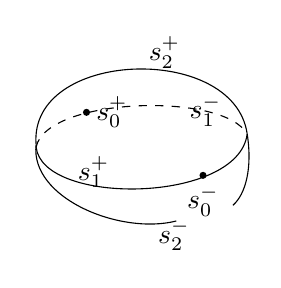
\begin{tikzpicture}[x=1cm,y=1cm]
\draw (0,0.05) .. controls (-.1,1.26) and (2.51,1.35) .. (2.68,.19) .. controls (2.75,-.25) and (2.66,-.58) .. (2.5,-.72);
\draw (0,.05) .. controls (-.08,-.63) and (1.07,-1.10) .. (1.78,-.92);
\draw (0,.02) .. controls (.08,-.73) and (2.56,-.70) .. (2.68,.18);
\draw[dashed] (0,.02) .. controls (.14,.66) and (2.41,.72) .. (2.68,.18);
\fill (.64,.46) circle (.045) node[right] {$s_0^+$};
\fill (2.12,-.34) circle (.045) node[below] {$s_0^-$};
\node at (.73,-.30) {$s_1^+$}; \node at (2.15,.48) {$s_1^-$};
\node at (1.63,1.22) {$s_2^+$}; \node at (1.75,-1.1) {$s_2^-$};
\end{tikzpicture}}

\deleted{\unsure{soit|$Z$}}

\diagram{\begin{tikzcd}[ampersand replacement=\&,row sep=small,column sep=small]
s_2^-\&s_2^+\&\\
s_1^-\arrow[u]\arrow[ur]\&s_1^+\arrow[u]\arrow[ul]\& =\unsure{\overline I|I|\overline J}\\
s_0^-\arrow[u]\arrow[ur]\&s_0^+\arrow[u]\arrow[ul]\&
\end{tikzcd}}

et l'antipodisme échange $s_i^-$ et $s_i^+$, mais le \deleted{groupe} quotient n'est pas ordonné, c'est la catégorie (\deleted{qui} importante pour la théorie des 2-Catégories)

% archive sheet number: 87
\scanpage{89}
\mspage{95}

\diagram{\begin{tikzcd}[ampersand replacement=\&,row sep=large]
s_2\\
s_1\arrow[u,shift left=1.8pt,"p_1^{\deleted{\unsure{-|+|*}}}" ]\arrow[u,shift right=1.8pt,"p_1^+"' ]\\
s_0\arrow[u,shift left=1.8pt,"p_0^{\deleted{\unsure{-|+}}}" ]\arrow[u,shift right=1.8pt,"p_0^+"' ]
\end{tikzcd}}

avec

\[
\left\{\begin{aligned}p_1^-p_0^-&=p_1^-p_0^+\\p_1^+p_0^-&=p_1^+p_0^+\end{aligned}\right.
\]

\deleted{Mais prenons le produit de $I$ par le \deleted{\unsure{ens.}} \inserted{groupoïde trivial} à deux éléments \deleted{\unsure{$0,1$}}\inserted{$\{0,1\}$}, sur lequel $G$ opère librement,}

Mais prenons la subdivision barycentrique de la décomposition cellulaire précédente de $S$ \deleted{soit} dont les sommets correspondent aux \inserted{éléments de $\mathrm{Ob}\,I$, les simplexes, aux} parties totalement ordonnées de $\mathrm{Ob}\,I$. On trouve l'\uline{octaèdre}

\figure{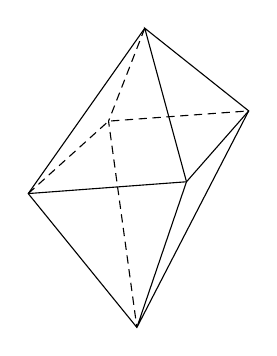
\begin{tikzpicture}[x=1cm,y=1cm]
\coordinate (t) at (1.48,2.1); \coordinate (b) at (1.38,-1.7);
\coordinate (l) at (0,0); \coordinate (r) at (2.8,1.05);
\coordinate (f) at (2.01,.15); \coordinate (h) at (1.02,.92);
\draw (t)--(l)--(b)--(r)--(t)--(f)--(b);
\draw (l)--(f)--(r); \draw[densely dashed] (t)--(h)--(b) (l)--(h)--(r);
\end{tikzpicture}}

\deleted{ayant 8 faces, \unsure{$4\times$}} ayant

\[
\begin{aligned}6&\text{ sommets}\\12&\text{ arêtes}\\8&\text{ faces}\end{aligned}
\]

et $G$ opère librement sur l'ens des simplexes, donc le quotient :

\[
\begin{aligned}3&\text{ sommets}\\6&\text{ arêtes}\\4&\text{ faces}\end{aligned}
\]

décomposition cellulaire du plan projectif. (Sa décomposition par trois droites.)

\figure{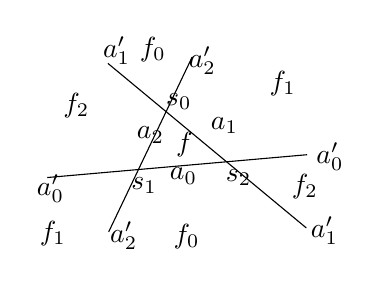
\begin{tikzpicture}[x=1cm,y=1cm]
\draw (-1.62,-.25)--(1.68,.04); \draw (-.84,-.94)--(.22,1.28); \draw (-.85,1.20)--(1.67,-.89);
\node at (-1.58,-.39) {$a'_0$}; \node at (1.97,.02) {$a'_0$};
\node at (-.74,1.36) {$a'_1$}; \node at (1.90,-.92) {$a'_1$};
\node at (.35,1.23) {$a'_2$}; \node at (-.65,-.99) {$a'_2$};
\node at (.05,.72) {$s_0$}; \node at (-.39,-.35) {$s_1$}; \node at (.81,-.25) {$s_2$};
\node at (.11,-.23) {$a_0$}; \node at (.63,.41) {$a_1$}; \node at (-.31,.29) {$a_2$};
\node at (.12,.17) {$f$}; \node at (-.28,1.38) {$f_0$}; \node at (.15,-1) {$f_0$};
\node at (1.37,.94) {$f_1$}; \node at (-1.55,-.96) {$f_1$};
\node at (-1.25,.67) {$f_2$}; \node at (1.65,-.36) {$f_2$};
\end{tikzpicture}}

On prend $S^1_{\deleted{\unsure{G|B}}}$ par l'ens. ordonné (comme au début)

\diagram{\begin{tikzcd}[ampersand replacement=\&,row sep=small,column sep=small]
s_1^-\&s_1^+\\ s_0^-\arrow[u]\arrow[ur]\&s_0^+\arrow[u]\arrow[ul]
\end{tikzcd}}

i.e.

\diagram{\begin{tikzcd}[ampersand replacement=\&,row sep=tiny,column sep=small]
\&s_1^+\&\\0=s_0^-\arrow[ur]\arrow[dr]\&\&s_0^+=0'\arrow[ul]\arrow[dl]\\
\&s_1^-\&
\end{tikzcd}}

et $G$ y opère, par symétrie échangeant $s_1^-$ et $s_{\unsure{1|i}}^+$. Donc \inserted{l'ens. ordonné} $X$ aura $4\times13=52$ sommets --- c'est \unsure{modeste|embêtant}\ldots

\figure{\begin{tikzpicture}[x=1cm,y=1cm]\draw (0,0) .. controls (.16,-.4) and (.55,-.87) .. (.83,-1.35); \draw (.68,-1.08)--(.66,-1.31);\end{tikzpicture}}

% archive sheet number: 88
\scanpage{90}
\mspage{96}

Finalement, il semble qu'il ne reste plus rien de la proposition 2 (p. 79) introduisant la notion de $\mathbb D$-fibration --- pas même l'équivalence des deux conditions b) et b') ($\mathbb D$-fibration à gauche universelle, $\mathbb D$-fibration à droite universelle). On songe à les relier à une condition a) modifiée ainsi (pour $f:X\unsure{\relbar|\to}Y$

a) Pour tout $Y''\to Y'\to Y$, avec $Y'$ et $Y''$ $\mathrm{Hot}$-\uline{asphériques} (et pas seulement $\mathbb D$-asphériques) $X''=X\times_Y Y''\longrightarrow X'=X\times_Y Y'$ est une $\mathbb D$-équivalence.

(Quand on suppose que $Y''$ et $Y'$ ont des éléments finaux, c'est la condition que $f$ soit une $\mathbb D$-fibration à gauche universelle ; quand on suppose que $Y''$ et $Y'$ ont des éléments initiaux, c'est la condition $\mathbb D$-fibration à droite universelle.)

% slanted
\margin{Il faut expliciter les raisonnements. Il suffit de tester même avec $Y''\unsure{\Rightarrow|\to}Y'$, où $Y''$ est \uline{ponctuelle}, et où $Y'$ a un objet final (resp. initial).}

On a évidemment

\diagram{\begin{tikzcd}[ampersand replacement=\&,row sep=small,column sep=small]
\&a\arrow[dl,Rightarrow]\arrow[dr,Rightarrow]\&\\b\&\&b'
\end{tikzcd}}

et on aimerait que ce soient des équivalences.

Voici un axiome \unsure{intéressant|intéress.} sur $\mathbb D$, qui \unsure{me} semble vérifié dans tous les cas connus, qui assure l'équivalence souhaitée. Je vais \deleted{\unsure{Der}}\inserted{en} \unsure{même} temps reformuler $\mathrm{Der}\,3$ en trois volets (cf p. \unsure{67|61}) ---

% slanted
\margin{cf \uline{$\mathrm{Der}$} 3 \unsure{a'|$\varphi'$}) page suivante}

% archive sheet number: 89
\scanpage{91}
\mspage{97}

\uline{Der 3} \textcircled{\scriptsize a} \deleted{\unsure{Soit}}\unsure{Si} $Z\in\mathrm{Diag}$ est $\mathrm{Hot}$-asphérique, alors $Z\xrightarrow{p}e$ est une $\mathbb D$-équivalence, i.e. $\inserted{p^*:}\underset{\shortparallel\, A}{\mathbb D(e)}\unsure{\relbar\joinrel\relbar|\to}\mathbb D(Z)$ est pl. fidèle.

\textcircled{\scriptsize b} (\deleted{\unsure{Renforce}}\inserted{Généralise} \textcircled{\scriptsize a}) Soit $f:Z\to Z'$ une flèche dans $\mathrm{Diag}$. Si $f$ est une $\mathrm{Hot}$-équivalence, c'est une $\mathbb D$-équivalence (i.e. $f^*:\mathbb D(Z')\to\mathbb D(\unsure{Z|2})$ induit une \uline{équivalence} entre les sous-catégories de $Z,Z'$ formées des objets constants)

\textcircled{\scriptsize a'} (Précise considérablement a) Si $Z\in\mathrm{Diag}$ est $\mathrm{Hot}$-asphérique, alors \inserted{on a \textcircled{\scriptsize a}, et} l'image \inserted{essentielle} de $\mathbb D(e)=A$ dans $\mathbb D(Z)$ est formée des objets \uline{localement constants} de $Z$, i.e. \inserted{des objets $F$} tels que le foncteur

\[
\unsure{\relbar}\qquad Z^{\unsure{o|\circ}}\longrightarrow A\qquad z\longmapsto F_z
\]

soit localement constant (i.e. transforme tte flèche en iso), donc \inserted{isom. à un foncteur} constant (puisque $Z$ est $\mathrm{Hot}$-asphérique, donc 1-connexe).

Il faut bien noter que dans a'), il ne \unsure{suffira|suffirait} \uline{pas} de supposer que $Z$ soit $\mathbb D$-asphérique, au lieu de $\mathrm{Hot}$-asphérique. Dès que la $D$-équivalence est \inserted{effectivement} plus faible que $\mathrm{Hot}$, il semble que \textcircled{\scriptsize a'} devienne \inserted{\unsure{toujours}} \deleted{\unsure{faux}} \unsure{f.} si on y \deleted{\unsure{remplace}} suppose seulement que $Z$ soit $\mathbb D$-asphérique. P. ex. même si $\mathbb D=\unsure{\mathbb D_i|\mathbb D_1|D_i}$ (théorie des \unsure{$i$|1}-types d'homotopie \unsure{relative|relatifs}), la \deleted{\unsure{condition}}\inserted{catégorie} \deleted{d'un objet \inserted{local. constant} de $\mathbb D(Z)$}

% slanted
\margin{\unsure{ou sous|ou tout} \unsure{quelles|quel} conditions sur $\mathbb D$ ?}

% archive sheet number: 90
\scanpage{92}
\mspage{98}

des objets localement constants sur $Z$ s'exprime en termes du $(i+1)$-type d'homotopie, mais pas en termes de son $i$-type d'homotopie \unsure{seulement}.

Il semble bien que ce soit l'axiome \uline{Der 3} (a') qui assure l'existence d'une bonne notion \inserted{(``\unsure{bilatér.|bilatère}'')} de $\mathbb D$-fibration, qui soit stable par changement de base, et qui se réduise soit à ``$\mathbb D$-fibration à gauche universelle'', soit à ``$\mathbb D$-fibration à droite universelle'' --- donc qui soit en plus \inserted{une condition} \uline{vérifiable} pratiquement.

Dans le cas où $f$ est propre ou lisse, le critère est particulièrement simple, puisqu'il se borne à la condition que \deleted{\unsure{pour}} les $f_*f^*\deleted{\unsure{A}}a_Y$, resp\textsuperscript{t.} les $f_!f^*a_Y$ \inserted{(pour $a\in A$)}, soient des objets loc. constants sur $Y$ (donc \uline{constants} si $Y$ est \uuline{Hot}-asphérique, en vertu de \unsure{Der,|Der} 3 a').

Je vais également introduire une variante \deleted{\unsure{de}} forte de \uline{Der} 3 b) :

% slanted
\margin{\uline{Der 3} $b'_0$ : le foncteur est fidèle \unsure{(??)|(?)} $b'_1$ : le foncteur est pl. fidèle $b_2$ : le foncteur \unsure{est} une équiv.}

\uline{Der 3} b') Soit $Z'\unsure{\relbar|\to}Z$ une $\mathrm{Hot}$-équivalence dans $\mathrm{Diag}$. Alors $f^*:\mathbb D(Z')\unsure{\relbar|\to}\mathbb D(\unsure{Z|2})$ induit une équivalence entre les catégories des \deleted{\unsure{objets}}coeff. \uline{loc. constants} sur $Z$ et sur $Z'$.

% archive sheet number: 91
\scanpage{93}
\mspage{99}

Dans certaines questions il suffira de savoir que ledit foncteur est pleinement fidèle. Cela \deleted{équivaut sans doute}\inserted{implique} \deleted{à dire} que

\[
H^{\unsure{\cdot|i}}_{\mathbb D}(Z,F)\overset{\sim}{\unsure{\relbar|\longrightarrow}}H^{\cdot}_{\mathbb D}(Z',f^*F)
\]

quand $F$ est \uline{loc.} \uline{constant} sur $Z$ \deleted{et} \deleted{\unsure{(quelle)}} (mais il n'est pas clair que cette condition implique tjrs la pleine fidélité), de $=$ pour l'homologie

\[
H^{\mathbb D}_{\cdot}(Z',\unsure{f'|f^*}F)\longrightarrow H^{\mathbb D}_{\cdot}(Z,F)
\]

% slanted
\margin{Mais c'est OK si on a des $\mathrm{Hom}$ internes dans les $\mathbb D(Z)\ \text{loc. const.}$, satisfaisant $\mathrm{Hom}(F,G)\simeq\mathrm{Hom}_{\unsure{C|e}}(e_Z,\mathrm{Hom}(F,G))$, où $e$ est l'élément final de $A$, les $\mathrm{Hom}$ devant \unsure{compatibles} aux images inverses.}

% slanted
\margin{On \unsure{pourra|pourrait} dire que $f:Z'\to Z$ est \deleted{alors} $\mathbb D$-équiv. \uline{0-complète} \uline{à gche}}

% slanted
\margin{et \deleted{\unsure{à droite}}\inserted{0-complète} \uline{à droite} dans le cas homologique.}

Moyennant cette condition, on a la

\uline{Proposition} : \inserted{On suppose \uline{Der} 3 b' satisfait} Soit $f:X\to Y$ dans $\mathrm{Diag}$. Pour que $f$ soit une $\mathbb D$-fibration, il f. et s. que pour $Y''\xrightarrow{p}Y'$ sur $Y$ qui soit une $\mathrm{Hot}$-équivalence, $X''=X\times_Y Y''\unsure{\relbar|\to} X'=X\times_Y Y'$ soit \deleted{une} $\mathbb D$-équivalence.

À vrai dire, on peut énoncer quelque chose de raisonnable, sans supposer l'axiome Der 3 b'. On doit introduire la

\uline{Définition} : Soit $f:Z'\unsure{\relbar|\to}Z$ dans $\mathrm{Diag}$. On dit que $f$ est une $\mathbb D$-équivalence 1-\uline{complète} si le foncteur $f^*:\mathbb D(Z)\unsure{\relbar|\to}\mathbb D(Z')$ est pleinement fidèle sur la sous-catégorie pleine de $\mathbb D(Z)$ formée des coeff\textsuperscript{ts} \uuline{loc.} constants. On dit que $f$ est une $\mathbb D$-équivalence 2-\uline{complète} si elle induit une équiv. entre les cat. de coeff\textsuperscript{ts} loc. constants.

% archive sheet number: 92
\scanpage{94}
\mspage{100}

On dit que $Z$ est \uline{complètemt} $\mathbb D$-\uline{asphérique}, si $Z\longrightarrow e$ est une $\mathbb D$-équivalence 2-complète.

Ainsi, l'axiome Der 3 \unsure{a''|a'}) peut \deleted{\unsure{se|s'être}} reformuler, en disant que si $Z$ est $\mathrm{Hot}$-asphérique, alors $Z$ est complètement $\mathbb D$-asphérique. On peut alors donner une variante affaiblie, qui suffira pour donner une notion raisonnable de $\mathbb D$-fibration :

% slanted
\margin{Et de $=$, Der 3 b', en disant que si $f:X\to Y$ \deleted{de} $\unsure{\in|\leftarrow}\mathrm{Diag}$ est une $\mathrm{Hot}$-\unsure{équiv.}, alors $f$ est une $\mathbb D$-équivalence 2-complète.}

\uline{Der 3} \unsure{b''|a''}) Toute $Z$ de $\mathrm{Diag}$ qui a soit un objet final, soit un objet initial, est complètement $\mathbb D$-asphérique.

\uline{Définition} On dit que $f:X\to Y$ dans $\mathrm{Diag}$ est une $\mathbb D$-fibration, si pour

\[
Y''\unsure{\relbar|\to}Y'\unsure{\relbar|\to}Y,
\]

avec $Y''\to Y'$ \deleted{\unsure{comme}} une $\mathbb D$-équivalence 1 complète (p. ex. $Y'$ et $Y''$ complètement $\mathbb D$-asphériques), $X''=X\times_Y Y''\unsure{\relbar|\to}X'=X\times_Y Y'$ est une $\mathbb D$-équivalence.

Cela équiv. à \deleted{\unsure{aux}}\inserted{chacune des} conditions b), b') de prop. 2. (page 79), i.e. que $f$ soit universellement $\mathbb D$-fibrant à gauche, ou $f$ univ. $\mathbb D$-fibrant à droite (grâce à Der 3 b'').

% archive sheet number: 93
\scanpage{95}
\mspage{101}

\uline{Définition 1} $f:X\to Y$ dans $\mathrm{Diag}$ est appelé $\mathbb D$-\uline{équivalence cohomologique} (sous-entendu : \uline{complète}) si pour tout $F\deleted{\unsure{\in\mathrm{Ob}|\in}}\mathbb D(Y)$, $F$ \uline{loc. constant}, on a

\[
H^{\cdot}_{\mathbb D}(Y,F)\xrightarrow{\sim} H^{\cdot}_{\mathbb D}(X,\unsure{f|f^*}(F))
\]

Notion duale $\mathbb D$-\uline{équivalence homologique}

\[
H^{\mathbb D}_{\cdot}(X,\unsure{f^*|f}(F))\xrightarrow{\sim}H^{\mathbb D}_{\cdot}(Y,F).
\]

Si $Y$ est \deleted{\unsure{total|tota}}\unsure{plètement|complètement} $\mathbb D$-asphérique, alors les coeff loc constants \inserted{sur $Y$} sont constants, et $f$ est une $\mathbb D$-équiv. coh. \inserted{(ou hom.)} \unsure{ssi|si} c'est une $\mathbb D$-équivalence, i.e. si $X$ est $\mathbb D$-asphérique.

% margin note written sideways
\margin{L'axiome \uline{Der} 3 b'$_1$ implique que toute $\mathrm{Hot}$-équivalence est une $\mathbb D$-équiv. cohom.}

\uline{Prop. 1} \inserted{(sorites)} : Soient $X\xrightarrow{f}Y\xrightarrow{g}Z$. Si $f$ et $g$ sont des $\mathbb D$-équivalences coh, alors $gf$ aussi ; si $gf$ et $f$ sont des $\mathbb D$-équiv. coh, alors $g$ aussi. Si $gf$ est une $\mathbb D$-équiv$^{\mathrm{ce}}$ coh, et si $g$ est une $\mathbb D$-équiv. \uline{2-complète} (donc tout $F$ loc constant sur $Y$ provient d'un $G$ loc constant sur $Z$), alors $f$ est une $\mathbb D$-équiv. coh.

\uline{Définition 2} : 1°) $f:X\to Y$ dans $\mathrm{Diag}$ est \deleted{appelé} une $\mathbb D$-\uline{fibration cohomologique} \inserted{(\deleted{\unsure{stricte|absolue}}\uuline{complète})}, je dis bien \uuline{complète} si

a) $\forall\,y\in\mathrm{Ob}\,Y$, $X_y\unsure{\relbar|\to}X_{/y}$ est une $\mathbb D$-équiv. \deleted{1-complète} cohomologique (complète)

b) $\forall\,y'\to y$ dans $Y$, $X_{/y'}\unsure{\relbar|\to}X_y$ est une $\mathbb D$-équiv. \deleted{1 complète} cohomologique (complète)

% archive sheet number: 94
\scanpage{96}
\mspage{102}

c) Ces conditions restent satisfaites après tout changement de base $Y'\to Y$.

2°) Notion duale de fibration homologique complète.

\uline{Exemple} Si $f$ est $\mathrm{Hot}$-propre, les \deleted{conditions}\inserted{flèches de} a) et b) sont des $\mathrm{Hot}$-équivalences, donc en vertu de Der 3 b'$_1$ (qu'il faut admettre) ce sont des $\mathbb D$-équiv. coh\unsure{om.|om}, \deleted{\unsure{ceci|cela}} signifie que a) et b) sont valables, et c) aussi car la notion de flèche $\mathrm{Hot}$-propre est stable par chgt. de base.

\uline{Prop 2} \deleted{\unsure{Soit $t$|Soient}} $\bar f:X\unsure{\relbar|\to}Y$ $\mathbb D$-fibration coh. complète, $F\in\mathrm{Ob}\,\mathbb D(X)$ loc constant sur $X$. Alors $f_*(F)$ est loc. constant, sa formation commute à tout chgt. de base, et en particulier se calcule \deleted{\unsure{fib}}\unsure{fibre|fibres} par fibres.

% slanted
\margin{il y a une réciproque cf prop 3 !}

\uline{Cor. 1} Soit \deleted{\unsure{alors|un}} un diagramme cartésien

\diagram{\begin{tikzcd}[ampersand replacement=\&,column sep=large]
{} \& X\arrow[d,"f"] \& X'\arrow[l,"q"']\arrow[d,"f'"]\\
\deleted{\unsure{Y'|Y}}\arrow[r,dash] \& Y \& Y'\arrow[l,"\unsure{p|g}"]
\end{tikzcd}}

On suppose $f$ $\mathbb D$-fibration cohomologique, et $p$ une $\mathbb D$-équiv. coh. Alors $q$ est une $\mathbb D$-équiv. coh.

% archive sheet number: 95
\scanpage{97}
\mspage{103}

En effet, on a pour $F$ loc. constant sur $X$

\[
\begin{aligned}
H^{\unsure{\cdot|i}}_{\mathbb D}(X,F)&\simeq H^{\cdot}_{\mathbb D}(Y,\underbrace{f_*(F)}_{\substack{\text{loc}\\\text{const. sur}\\Y}})
\xrightarrow[\substack{|\\ p\ \mathbb D\text{-équ.}\\\text{coh}}]{\sim}
H^{\cdot}_{\mathbb D}(Y',\underbrace{\unsure{p'|p^*}f_*(F)}_{\substack{\rotatebox{90}{$\simeq$}\\ f'_*q^{\unsure{*|\prime}}(F)\\\text{par prop. 2}}})\\
&\simeq H^{\cdot}_{\mathbb D}(Y',f'_*q^*F)\simeq H^{\cdot}_{\mathbb D}(X',q^*F)
\end{aligned}
\]

qed.

\uline{Prop 3} La notion de $\mathbb D$-fibration cohomologique \inserted{complète} est stable par chgt de base (trivial) et par composition.

\deleted{Il suffit de prouver les conditions a), b) pour $gf$ dans $X\xrightarrow{f}Y\xrightarrow{g}Z$.} Pour la stabilité par composition, il suffit de \deleted{\unsure{voir}} noter le cor. suivant de prop. 2

\uline{Cor. 2} (de Prop. 2) Soit $f:X\to Y$. Pour que $f$ soit une $\mathbb D$ fibration cohomologique \inserted{complète}, il f. et s. que pour $Y''\xrightarrow{\unsure{p'|p}}Y'\to Y$ \unsure{sur $Y$}, avec $p$ une $\mathbb D$-équiv coh, la flèche correspondante $X''=X\times_Y Y''\unsure{\relbar|\to}X'=X\times_Y\unsure{Y/|Y'}$ soit aussi une $\mathbb D$-équiv coh.

C'est nécessaire par le cor. 1, compte tenu que $f':X'=X\times_Y Y'\unsure{\relbar|\to}Y'$ \deleted{est} aussi une $\mathbb D$-fibr. coh. C'est suffisant, car il suffit de l'appliquer aux cas $\{y\}\unsure{\relbar|\to}Y_{/\{y\}}$, $\deleted{\unsure{\Rightarrow|y}}Y_{/\,\unsure{,y|y}}\unsure{\relbar|\to}Y_{/y'}$, qui sont des $\mathbb D'$-équiv. coh. en

% archive sheet number: 96
